\section{Exercise two}

Consider the system: 
\[\begin{cases}
    x_1(t+1)=\dfrac{1}{2}x_1(t)+v_{11}(t) \\
    x_2(t+1)=2x_2(t)+v_{12}(t) \\
    y(t)=x_2(t)+v_2(t)
\end{cases}\]
Where: 
\begin{itemize}
    \item $v_1(t)=\begin{bmatrix} v_{11}(t) \\ v_{12}(t) \end{bmatrix} \sim WN\left(\begin{bmatrix} 0 \\ 0 \end{bmatrix},\begin{bmatrix} 1 & 0 \\ 0 & 1 \end{bmatrix}\right)$. 
    \item $v_2(t)\sim WN(0,1)$.
    \item $v_1(t)$ is independent from $v_2(t)$. 
\end{itemize}
\begin{enumerate}
    \item Draw the block scheme. 
    \item Check if the asymptotic state prediction error is bounded.
    \item Compute the steady state predictor using the two subsystems.
    \item Find the transfer function from $y(t-1)$ to $\hat{x}_2(t|t)$. 
\end{enumerate}

\subsection*{Solution}
\begin{enumerate}
    \item The block scheme is depicted below:
        \begin{figure}[H]
            \centering
            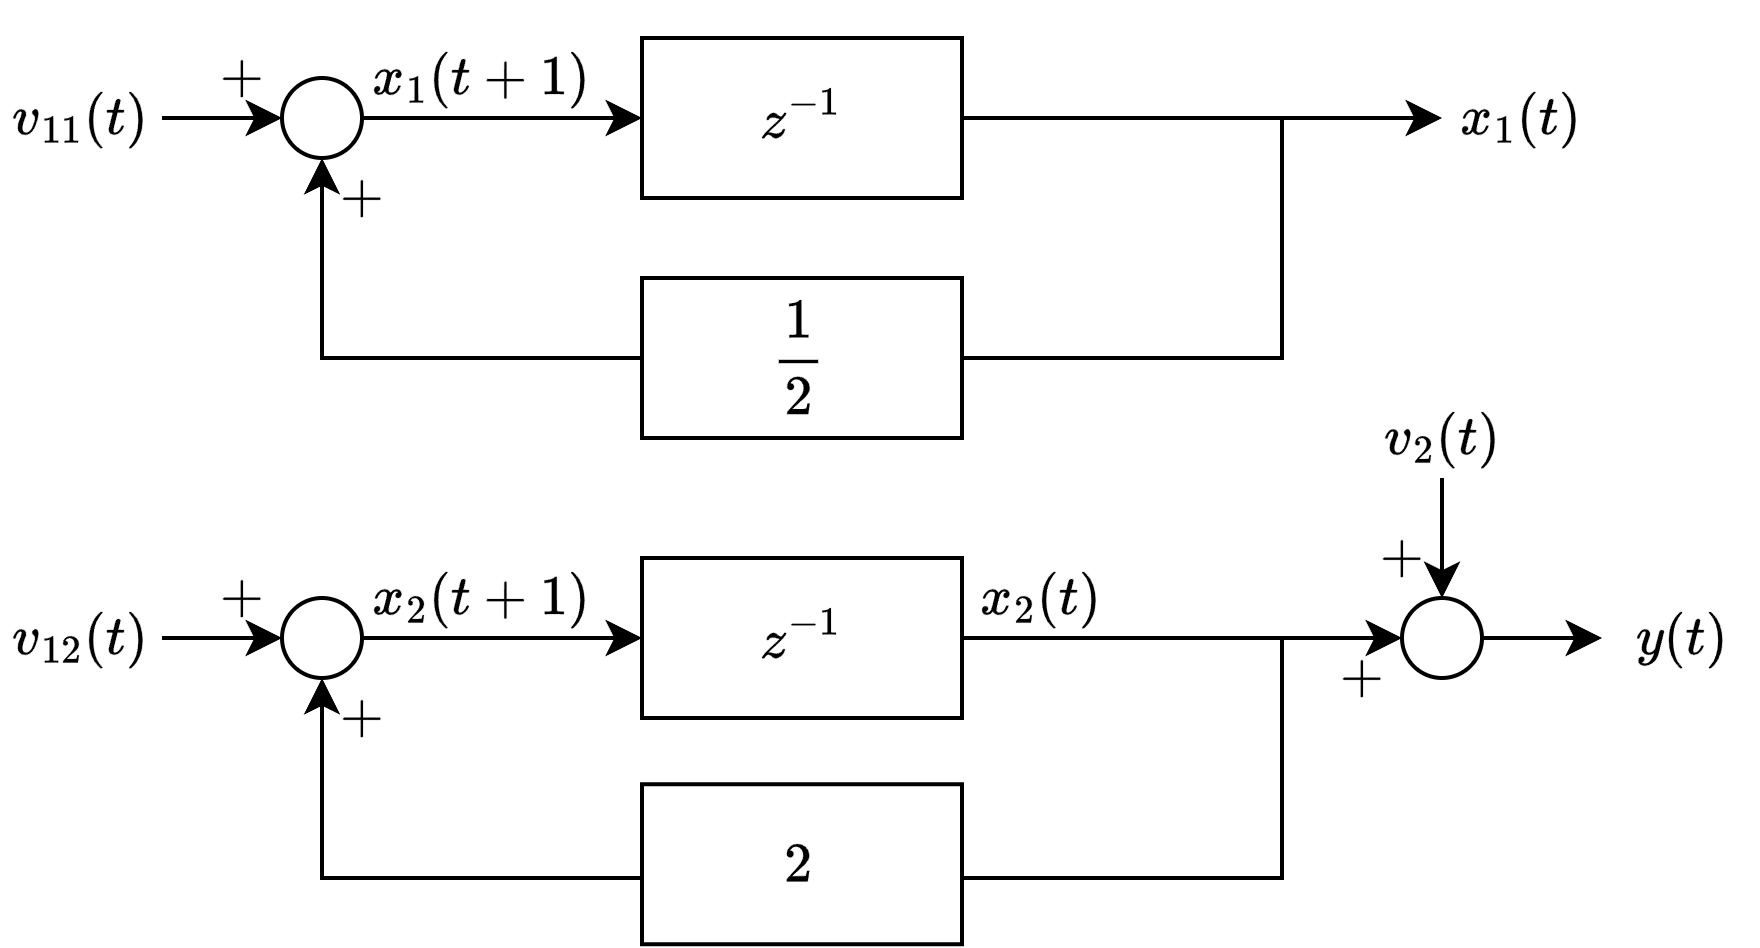
\includegraphics[width=0.75\linewidth]{images/ex1.png}
        \end{figure}
    \item A system is considered bounded if it is either asymptotically stable or simply stable. 
        Let's analyze the system using the two theorems for Kalman filters.
        For the first theorem we have: 
        \begin{itemize}
            \item $V_{12}=0$
            \item The system is asymptotically stable if its poles are inside the unit circle.
                In this case the poles are $z_{1,2}=\frac{1}{2},2$, indicating that the system is not asymptotically stable.
        \end{itemize}
        Due to one unmet hypothesis, the first theorem cannot be applied.

        For the second theorem we have: 
        \begin{itemize}
            \item $V_{12}=0$
            \item $(F,H)$ is observable. 
                The observability matrix is: 
                \[O=\begin{bmatrix} 0 & 1 \\ 0 & 2 \end{bmatrix}\]
                So the system is not fully observable. 
        \end{itemize}
        Since one hypothesis is not satisfied, the second theorem cannot be applied.

        Given that the system's states are uncoupled, we can decompose the system into two subsystems:
        \[\begin{cases}
            x_1(t+1)=\frac{1}{2}x_1(t)+v_{1A}(t) \\
            y_A(t)=0x_1(t)+\underbrace{v_{2A}(t)}_{\text{fictitious}} 
        \end{cases} \qquad
        \begin{cases}
            x_2(t+1)=2x_2(t)+v_{1B}(t) \\
            y_B(t)=x_2(t)+v_{2B}(t)
        \end{cases}\]
        For Subsystem A:
        \[F_A=\frac{1}{2}\quad V_{1A}=1\quad H_A=0 \quad V_{2A}=\varepsilon>0\quad V_{12A}=0\]
        For Subsystem B:
        \[F_B=2 \quad V_{1B}=1\quad H_B=1 \quad V_{2B}=1\quad V_{12B}=0\]

        We can now reapply the theorems to the two subsystems. 
        Beginning with theorem one for subsystem A:
        \begin{itemize}
            \item $V_{12A}=0$. 
            \item The system is asymptotically stable if the poles are inside the unit circle.
                In this case, the pole is $z=\frac{1}{2}$, indicating that the system is asymptotically stable.
        \end{itemize}
        Since all the hypotheses are satisfied, we can apply the first theorem, which asserts the existence of an asymptotic predictor.

        For subsystem B, we directly apply the second theorem since the first theorem cannot be applied due to the pole at $z=2$. 
        Here's the analysis:
        \begin{itemize}
            \item $V_{12B}=0$
            \item $(F,H)$ is observable. 
                The observability matrix is: 
                \[O=\begin{bmatrix} 1 \end{bmatrix}\]
                This indicates that the system is fully observable.
            \item To satisfy the condition $\Gamma\Gamma^T=V_{1B}=1$, we need $\Gamma=1$. 
                Therefore, the reachability matrix from noise is:
                \[R=\begin{bmatrix} 1 \end{bmatrix}\]
                Since it is full rank, it is reachable.
        \end{itemize}
        Since all the hypotheses are satisfied, we can apply the second theorem, which confirms the existence of an asymptotic predictor for subsystem B.

        In conclusion, the prediction error is bounded because each subsystem is asymptotically stable and has an asymptotic predictor.
    \item For the subsystem A: 
        \[\begin{cases}
            x_1(t+1)=\frac{1}{2}x_1(t)+v_{1A}(t) \\
            y_A(t)=0x_1(t)+\underbrace{v_{2A}(t)}_{\text{fictitious}} 
        \end{cases}\]
        We find the Kalman gain:
        \[\hat{K}_A=(F_A\bar{P}_AH_A+V_{12A})(H_A\bar{P}_AH_A^T+V_{2A})=\dfrac{0}{\varepsilon}\]
        Since the gain is null, no correction is applied to the prediction.

        For subsystem B:
        \[\begin{cases}
            x_2(t+1)=2x_2(t)+v_{1B}(t) \\
            y_B(t)=x_2(t)+v_{2B}(t)
        \end{cases}\]
        We solve the Algebraic Riccati Equation: 
        \[\bar{P}_B=F_B\bar{P}_BF_B^T+V_{1B}-\dfrac{\left(F_B\bar{P}_BH_B^T+V_{12B}\right)^2}{H_B\bar{P}_BH_B^T+V_{2B}}=\dfrac{5\bar{P}_B+1}{\bar{P}_B+1}\]
        The solutions are: 
        \[\bar{P}_B=2\pm\sqrt{5}\]
        The second solution is invalid because it's smaller than zero.

        We then compute the Kalman gain:
        \[\bar{K}_B=\left(F_B\bar{P}_BH_B^T+V_{12B}\right)\left(H_B\bar{P}_BH_B^T+V_{2B}\right)=\dfrac{4+2\sqrt{5}}{3+\sqrt{5}}\]
        Since $F_B-\bar{K}_BH_B=\dfrac{2}{3+\sqrt{5}}\approx 0.4$, the system is asymptotically stable.

        The predictor is:
        \[\hat{x}_2(t+1|t)=\dfrac{2}{3+\sqrt{5}}\hat{x}_2(t|t-1)+\dfrac{4+2\sqrt{5}}{3+\sqrt{5}}y(t)\]
    \item To find the filter from the predictor, we start with:
        \[\hat{x}(t+1|t)=(F-KH)\hat{x}(t|t-1)+Ky(t)\]
        Expanding this, we get:
        \[F\hat{x}(t|t)=(F-KH)F\hat{x}(t-1|t-1)+Ky(t)\]
        If $F$ is invertible, we can express $\hat{x}(t|t)$ as:
        \[\hat{x}(t|t)=(I-F^{-1}KH)F\hat{x}(t-1|t-1)+F^{-1}Ky(t)\]
        Substituting the given values, we have:
        \[\begin{cases}
            \hat{x}(t|t)=\begin{bmatrix}
                \frac{1}{2} & 0 \\ 0 & \frac{2}{3+\sqrt{5}}\end{bmatrix}\hat{x}(t-1|t-1)+\begin{bmatrix} 0 \\ \frac{4+2\sqrt{5}}{3+\sqrt{5}} \end{bmatrix} y(t) \\
                \hat{x}_2(t-1|t-1)=\begin{bmatrix} 0 & 1 \end{bmatrix}\hat{x}(t-1|t-1)
        \end{cases}\] 
        The transfer function from $y(t)$ to $\hat{x}_2(t-1|t-1)$ is: 
        \[W(z)=\tilde{H}(zI-\tilde{F})^{-1}\tilde{G}=\dfrac{4+2\sqrt{5}}{3+\sqrt{5}}\dfrac{1}{z-\frac{2}{3+\sqrt{5}}}\]
        So, we have:
        \[\hat{x}_2(t-1|t-1)=\dfrac{4+2\sqrt{5}}{3+\sqrt{5}}\dfrac{1}{z-\frac{2}{3+\sqrt{5}}}y(t)\]
        However, we need $y(t-1)$, so:
        \[W(z)=\dfrac{4+2\sqrt{5}}{3+\sqrt{5}}\dfrac{z}{z-\frac{2}{3+\sqrt{5}}}\]
\end{enumerate}